%\documentclass{sigchi}
\documentclass{article}



\usepackage{graphics} % for EPS, load graphicx instead
\begin{document}


\title{HabilisX: Document Exploration Through a Tool-Based Touch Screen Environment }
\author{Prairie Rose Goodwin}
\date{}
\maketitle
\begin{abstract}
This project explores a new touch screen interface for interacting with data sets through a digital tool metaphor.  Research in psychology has shown that when we hold a tool, such as a hammer, our minds frame potential solutions around the affordances of the tool.  Additionally, metaphors have proven to be a powerful way to positively affect user experience, in part because the user has expectations about how different objects behave.  Our system attempts to recreate the experience of using physical tools. Touch screens provide the ideal interaction style for this metaphor because they allow the user to be more physically engaged than a traditional point-and-click interaction. With the support of the James B. Hunt Library at North Carolina State University, we created a work environment with life-size tools using a 40-inch PixelSense 2.0 touch screen table.  Our interface consists of two and a half dimensional representations of paperclips, pushpins, rulers, magnifying glasses, "magic lenses", and sticky notes that can be used to manipulate database entries that appear as index cards scattered randomly on the table.  All objects on the screen have physical properties like center of mass, momentum, and friction to mimic the behavior of real objects on a table.  The tools are designed to let the user search and organize the data efficiently by taking advantage of spatial cognition and information visualizations.  Moreover, the user can leverage basic filtering queries by attaching "filter tiles" to the tools that dictate the entries with which the tools will interact.  Our goal is to show that our system is user-friendly and allows users to categorize data faster and more accurately than a comparable tabular interface.
\end{abstract}
\section{keywords}
Information Visualization, Spatial Cognition, Spatial Memory, Document Management, Database Interface

\section{Introduction}	

%Tool use is a fundamental aspect of the ways in which humans interact with their environments, bot in the physical world and within the computer interface. 
%
%Analogies in software environments follow naturally from our experience with tools in the real world.  
%
%The ubiquity and effectiveness of the tool metaphor in software environments suggest that people's experiences with everyday physical tools carries over to the use of software tools.  Yet little effort has been put into understanding the characteristics of physical tool use and how those characteristics may support or undermine interactions when adapted to software design.
%
%We believe that an improved understanding of the nature of tool use and its related concepts can help us to generate better explanations of why many software tools are effective.  Further, the application of these concepts can lead to the development of novel interaction techniques.  
%
%The separation between physical and cognitive tool use is not a sharp line;  
%
%
%The applications in this section illustrate how tools can influence design in domains that may  have less than obvious physical interpretations.
\section{Related Work} 
\subsection{Tool Metaphor}

GUI Metaphors allow users to represent problems in a more easily solvable format.  As cognitive tools defined by Hutchins \cite{Hutchins1995} and Norman \cite{Norman1991}, they have shown that they can be extremely powerful aids.  Since the introduction of the desktop metaphor by Xerox in the '70's  it has become ubiquitous for personal computers.  Command line usability is notoriously difficult for beginners and non-technical users, whereas being able to interact with visual icons gives users an underlying model of what their actions are doing.  This allowed a whole new demographic to use computers, and subsequently the adoption of home computers skyrocketed.  

This project explores a novel user interface with a tool metaphor for database searches.  Tool metaphors have been introduced at a surface level in some conventional software environments.  Most notably visual programs like photoshop or paint have a tools that have analogs to real world objects.  However, the metaphor is usually quite shallow, and beyond icon and task, bear little resemblance to the experience of using that tool.  This is important because there is a cognitive shift that occurs when using a physical tool in which the user starts to think of the tool as an extension of his or her body.  \cite{Maravita2004}  When we factor in the affordance of a tool, we realized that tool metaphors have the ability to remold the experience into something familiar.  

Direct manipulation interfaces provide a good environment to explore affordances in software \cite{Gaver1991}, \cite{Norman1991}.  Users interact directly with objects on the screen instead of with menus or commands \cite{Hutchins1989} \cite{Shneiderman1992}, which are continuously represented with animation instead of appearing and disappearing as needed.\cite{Shneiderman1992}  Getner argued that deeper metaphors that are more consistent with the physical world can improve learnability and usability of the system \cite{Gentner1996} and can be a good opportunity for the user to become familiar with the system \cite{Fischer1994}.  


\subsection{Spatial Cognition}
There is a large body of work that has shown the cognitive benefits of being able to organize items spatially. \cite{Agarawala2006} \cite{Robertson1998} Robertson et al. made a 2½-D interface for bookmarking website that showed dramatic improvement in efficiency and error over the built in text-based system.  
	
	Most work has been done between a graphical environment versus a textual environment, but Sebrechts et al took this concept one step further and did a formal evaluation of a text-based, 2-D, and 3-D interfaces.\cite{Sebrechts1999}  They found that the 2-D interface had the best performance in both user satisfaction and performance.  Additionally, they tried multiple input devices, which made a significant impact on the usability of the interface. 

\subsection{Touch}
Touch screens have become popular in recent years, but many feel that they are a step backwards in usability \cite{Norman2010}.  Gestures have many of the drawbacks of a command line interface: commands can be hard to remember, impossible to explore, and hard to debug.  There are no visual cues for what gestures the system will recognize, and there is not a standard set of gestures for all functionality.   Some work has been done to standardize gestures to make them more intuitive \cite{North2009}, but adoption of standards continues to be a problem with a few exceptions like pinch to zoom.  

	New work suggests that multi-touch interfaces may also have a usability gain for expert users when used appropriately. \cite{Forlines2007} \cite{Tan2002}\cite{North2009}.  It has less chance of causing carpal tunnel, and is more efficient in the amount of time to select targets than the mouse, which is the majority of screen interaction \cite{Forlines2007}.  Tabletop touch screen interactions showed that users benefited from direct touch input over mouse.  However, for traditional computers, some tasks were more efficiently done with a mouse. \cite{Kristensson2008}.  Moreover, using a table is a more active form or interaction because of the larger amount of movement required to reach the entire screen. This  full embodied interaction has shown  even more cognitive benefits. Kinesthetic signals (muscle memory) has been shown to improve spatial recall by 19\% in an experiment document retrieval setting.\cite{Tan2002} 


\subsection{Document Management}

So much of what we do with computers is dependent on being able to find pertinent information.  Many systems have focused on how to keep personal documents organized in a desktop interface with positive results \cite{Agarawala2006} \cite{Foo2007:ECDL} \cite{Foo2007:ICADL}. 

%\cite{Bier2005}

%This paper presents icon abacus, a space-efficient technique for displaying document attributes by automatic positioning of document icons. It displays the value of an attribute by using position on a single axis, allowing the other axis to display different metadata simultaneously The layout is stable enough to support navigation using spatial memory.

%no results posted


%\cite{Foo2007:ECDL}
%The task of searching for documents is becoming more challenging as the volumes of data stored continues to increase, and retrieval systems produce longer results list. Graphical visualisations can assist users to more efficiently and effectively understand large volumes of information. This work investigates the use of multiple visualisations in a desktop search tool. These visualisations include a List View, Tree View, Map View, Bubble View, Tile View and Cloud View. A preliminary evaluation was undertaken by 94 participants to gauge its potential usefulness and to detect usability issues with its interface and graphical presentations. The evaluation results show that these visualisations made it easier and quicker for them to find relevant documents. All of the evaluators found at least one of the visualisations useful and over half of them found at least three of the visualisations to be useful. The evaluation results support the research premise that a combination of integrated visualisations will result in a more effective search tool. The next stage of work is to improve the current views in light of the evaluation findings in preparation for the scalability and longitudinal tests for a series of increasingly larger result sets of documents.

%s. There was strong support 
%that they made it easier (83\%) and quicker (86\%) to find relevant documents. 


%\cite{Mothe1998}

 %INQUERY [l] proposes a graphical view of the retrieved documents where similar documents are graphically close; the retrieved docu- ments are listed to the user according to the class they belong to. VIBE [G] represents the information in a two dimensional space (document vs term) so that it is possible to graphically see which are the possible relevant documents according to some selected terms. Some complementary studies have shown that it is efficient to use the document structure or the factual information extracted from a document. ENVISION [5] represents the retrieved documents into two-dimensional tables. Rows and columns represent either factual information such as authors, date, or estimated relevance and cells are filled with document references, navigation through those ta- bles is possible. In this poster we propose an interactive document vi- sualization tool. It takes into account the fact that document relevance depends on the document features which are considered (information content, publication date, author affiliation, . ..). Those elements are crossed in order to discover the strong links that exist between them. Discovered relationships are then displayed on a 4-dimensional graphical view. This interface allows the user to graphically select the elements he is most inter- ested in and to automatically construct new filters that will change interactively the set of the displayed documents

%No results right nwo.. 
 
%\cite{Newman2010}
%This paper explores visualizations of document collections, which we call topic maps. Our topic maps are based on a topic model of the document collection, where the topic model is used to determine the semantic content of each document. Using two collections of search results, we show how topic maps reveal the semantic structure of a collection and visually communicate the diversity of content in the collection. We describe techniques for assessing the validity and accuracy of topic maps, and discuss the challenge of producing useful two-dimensional maps of documents.

%While not explored in this paper, we have the opportunity to use many visualization techniques to improve the usability and interpretability of our topic maps, beyond simple color coding by a single topic. We often have other attributes or metadata (such as authors, citation links and subject headings) that can enhance topic maps, using any combination of color, shape, size and text annotations.

%One conclusion from this work is that local topic maps (which dynamically show a few dozen closely related documents) may be more accurate. While topics are a useful way to organize an entire collection, producing a static global topic map of the collection may have limited value for exploring the collection. Therefore local topic maps may ultimately be more useful for better understanding and navigating local structure in a collection.


%\cite{Nowell1996}
%A digital library of computer science literature, Envision provides powerful information visualization by displaying search results as a matrix of icons, with layout semantics under user control. Envision’s Graphic View interacts with an Item Summary Window giving users access to bibliographic information, and XMosaic provides access to complete bibliographic information, abstracts, and full content. While many visualization interfaces for information retrieval systems depict ranked query-document similarity, Envision graphically presents a variety of document characteristics and supports an extensive range of user tasks. Formative usability evaluation results show great user satisfaction with Envision’s style of presentation and the document characteristics visualized.

%For the
%two benchmark subtasks using the Graphic View,
%participants made no errors, asked no questions, and all
%required less time than expected to complete the benchmark
%tasks — to our delight, surpassing the performance of an
%Envision designer!


%\cite{schraefel2002}
%Hunter Gatherer is an interface that lets Web users carry out three main tasks: (1) collect components from within Web pages; (2) represent those components in a collection; (3) edit those component collections. Our research shows that while the practice of making collections of content from within Web pages is common, it is not frequent, due in large part to poor interaction support in existing tools. We engaged with users in task analysis as well as iterative design reviews in order to understand the interaction issues that are part of within-Web-page collection making and to design an interaction that would support that process.We report here on that design development, as well as on the evaluations of the tool that evolved from that process, and the future work stemming from these results, in which our critical question is: what happens to users perceptions and expectations of web-based information (their web-based information management practices) when they can treat this information as harvestable, recontextualizable data, rather than as fixed pages?


%\cite{Shneiderman2000}
%Digital library search results are usually shown as a textual list, with 10-20 items per page. Viewing several thousand search results at once on a two-dimensional display with continuous variables is a promising alternative. Since these displays can overwhelm some users, we created a simplified two-dimensional display that uses categorical and hierarchical axes, called hieraxes. Users appreciate the meaningful and limited number of terms on each hieraxis. At each grid point of the display we show a cluster of color-coded dots or a bar chart. Users see the entire result set and can then click on labels to move down a level in the hierarchy. Handling broad hierarchies and arranging for imposed hierarchies led to additional design innovations. We applied hieraxes to a digital video library of science topics used by middle school teachers, a legal information system, and a technical library using the ACM Computing Classification System. Feedback from usability testing with 32 subjects revealed strengths and weaknesses.
%\cite{Yost2006}
%Larger, higher resolution displays can be used to increase the scalability of information visualizations. But just how much can scalability increase using larger displays before hitting human perceptual or cognitive limits? Are the same visualization techniques that are good on a single monitor also the techniques that are best when they are scaled up using large, high-resolution displays? To answer these questions we performed a controlled experiment on user performance time, accuracy, and subjective workload when scaling up data quantity with different space-time-attribute visualizations using a large, tiled display. Twelve college students used small multiples, embedded bar matrices, and embedded time-series graphs either on a 2 megapixel (Mp) display or with data scaled up using a 32 Mp tiled display. Participants performed various overview and detail tasks on geospatially-referenced multidimensional time-series data. Results showed that current designs are perceptually scalable because they result in a decrease in task completion time when normalized per number of data attributes along with no decrease in accuracy. It appears that, for the visualizations selected for this study, the relative comparison between designs is generally consistent between display sizes. However, results also suggest that encoding is more important on a smaller display while spatial grouping is more important on a larger display. Some suggestions for designers are provided based on our experience designing visualizations for large displays. Index Terms—Information visualization, large displays, empirical evaluation.
\section{Habilis}


Our system has a well established set of interaction mechanisms, and clear parallels to physical tools in the real world.

We propose a novel way to display and organize information visually through the metaphor of physical tools. Tool-use in the physical world generally includes an object in the operator's hand and broad motions to perform an action. We propose to extend these concepts to digital tools by implementing a program on the Microsoft Pixelsense 2.0 that lets the user select (pick-up) tools on the screen and perform motions that mimic physical tool usage. 
Program description:

\begin{figure}[t!]
\centering
\scalebox{.239}
{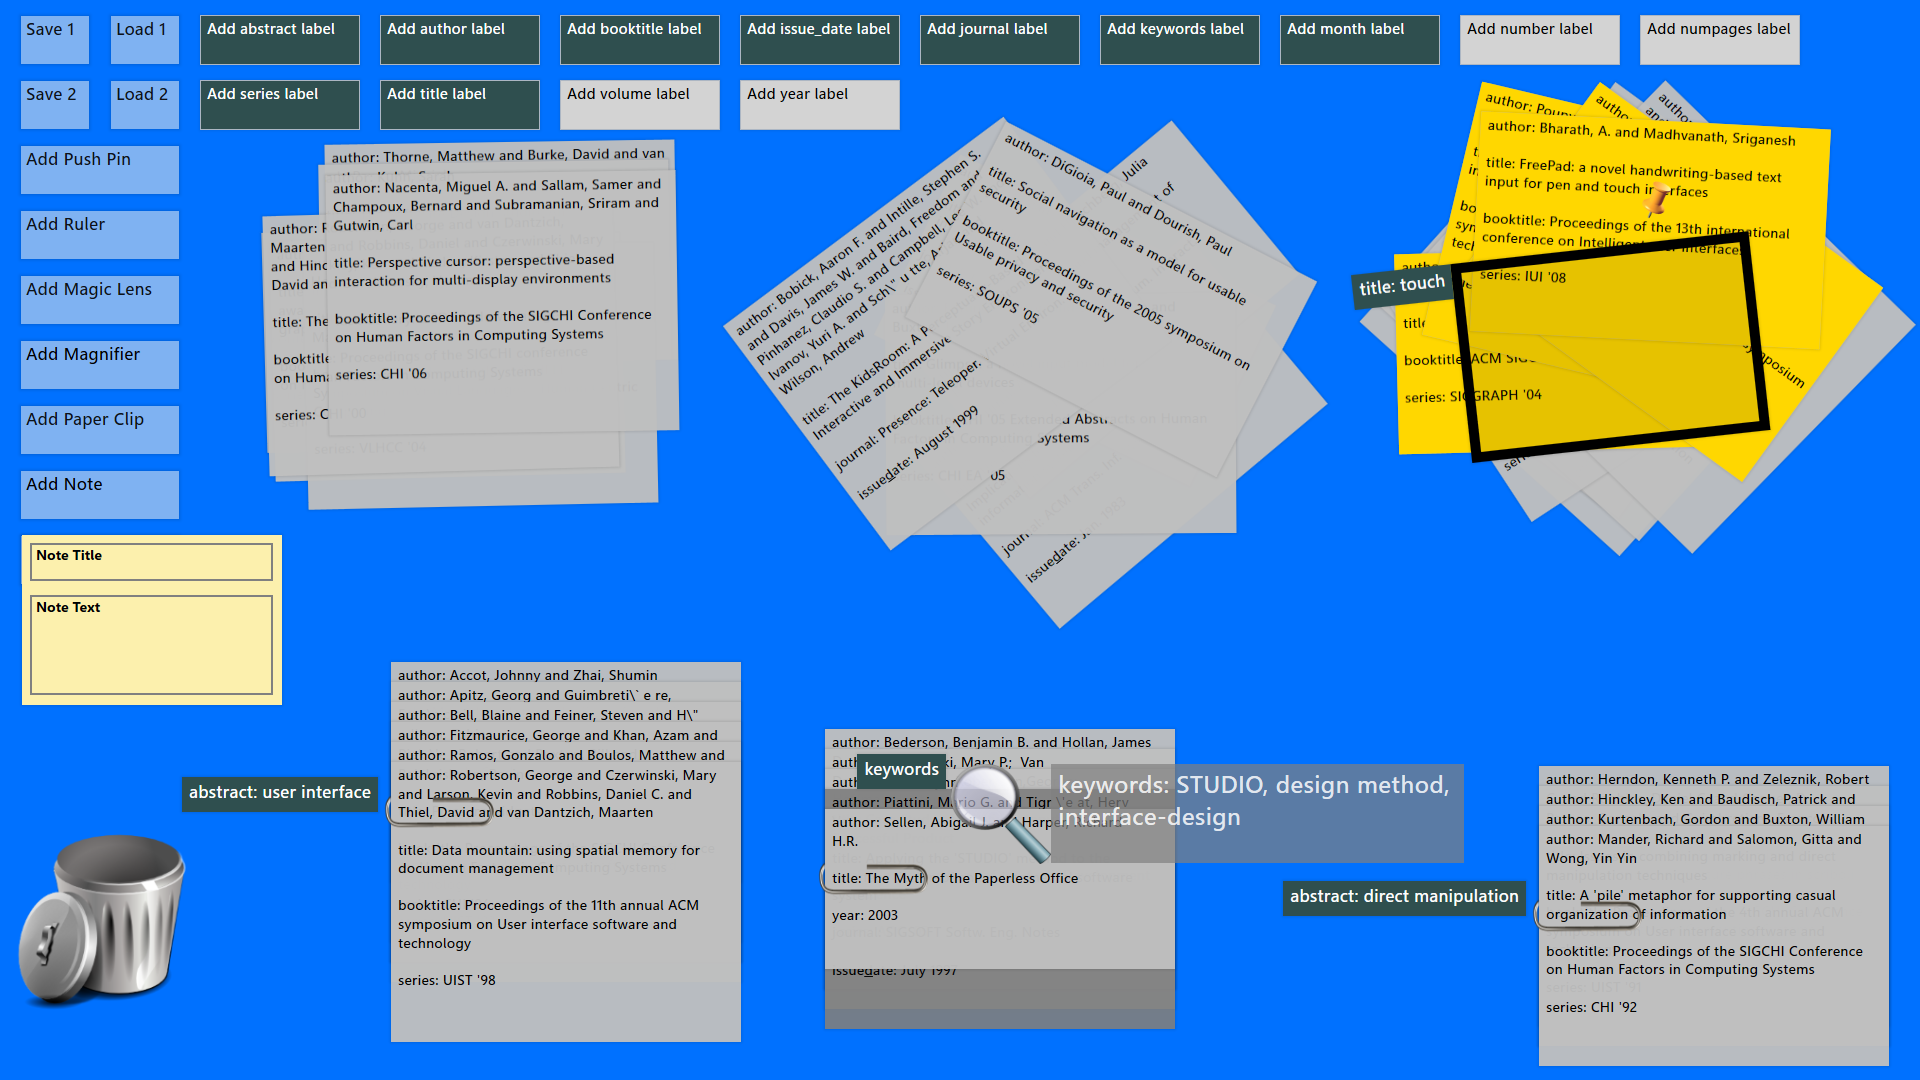
\includegraphics{HabilisScreenShot.png}}
\caption{Screenshot of Habilis after having used all tools.}
\label{Fig:screenshot}
\end{figure}



This program would be used to search and organize information stored in a database.  After getting an initial body of entries to search, each entry will appear as individual tiles with properties of naive physics that can be moved around the screen by touch. 






\subsection{Save States}
Habilis included two save states.  You can switch between two configurations of data for comparative purposes.  The tools do not change when a save state is loaded.  This is in part to maintain object permanence, but also so that the same queries can be used on either configuration.  

\subsection{Filter Tiles}
The name of each attribute or column header is shown on buttons that generate a label when pressed. These labels specify search criteria and can be attached to the tools to determine the items with which the tool will interact. For example, if the attribute is a string, the user should be able to specify a particular string to search for. If the attribute is an int, the user should be able to use any of the compare functions available such as greater than, less than, etc. 

Example: Let's say that your data set is a collection of research papers with the attributes: 

(String) Title
(String) Author
(Date object) DatePublished
(List<String>) Keywords
(int) pages

If you are looking for a paper on computer vision published in the last 5 years that is between 5 and 10 pages, you could create the query labels:
\begin{itemize}
\item Pages: $>$ 5
\item Pages: $<$ 10
\item Date: $<$ 2000
\item Keywords: "Computer Vision"

\end{itemize}

A single tool that has all of these queries would match to a paper that is 5-10 pages long, published before the year 2000, with the author- supplied keyword "Computer Vision".


Once created, you can attach and detach the query labels to tools by intersecting the two objects to quickly interact with your data.

\subsection*{Sticky Note}
Sticky Notes attach directly to entries and look similar to a filter with a different background color.  Once attached, the note will display the title, but tap it once to switch to the body of the note, and again to see the title again.
\subsection{Habilis Tools}
Not all tools can accept filters.  The focus of this project was searching, so the tools that were useful for that task cab accept filters. However, for other tasks, we found it was more useful to have tools that were consistent for all entries.  These tools were used for modifying entries based on their location rather than their content.   	
\subsection*{Push Pin}
The pushpin is used to "save" entries.  Once pinned, the entry is immobilized and no other tool can modify that entry.  Entries can be thrown under a pin to create a messy pile.  
\subsection*{Ruler}
The ruler can push entries around the screen and organize them visually by aligning them horizontally or vertically.  This state is somewhere in between a tidy pile and a messy pile as it does not afford browsing.  However, it unmistakably shows you entries that are categorized together.  
\subsection*{Trash Can}
The trashcan removes any unwanted entries or tools.  Just like in a Desktop GUI, just drag the item to the trash can, and it will disappear from the screen.  
\subsection{Habilis Filter Tools}
The following tools can be modified by attaching filter tiles.  Once attached, the tool will only interact with the entries that match the tile's query.  
\subsection*{Magic Lens}
The magic lens is a window that highlights entries that match your query.  Additionally, the lens will pop the results to the front of the interface so that no result is hidden.  
\subsection*{Magnifier}
The magnifier lets you view any attribute of an entry.  Simply drag the filter tile to the magnifier and instead of creating a query, the corresponding data of that attribute will be displayed in a pop-up next to the tool.  Drag any number of filter tiles, and the attribute will be displayed below the last one.  
\subsection*{Paper Clip}
Paper clips are used to create organized piles, or "tidy piles".  If no filters are attached, the paper clip will pick up everything.  If a filter tile is added, it will drop any entries that do not mach the query.  
%\subsection{Metaphor Structures}
%\subsection*{Messy Piles}
%\subsection*{Tidy Piles}
%like piles
\subsection{Habilis Interaction Design}
The buttons that were initially placed on the screen to populate the tools are not movable, scalable, or rotatable.  They can be activated by a quick or long touch and have no other interactions.  

All other UI Elements were sub-classed from a ScatterViewItem and have the same interaction properties.  All elements have have physical properties like center of mass, momentum, and friction to mimic the behavior of real objects on a table.  You can drag them around using one finger, but having two fingers on the tool disabled its use so that you could drag it around the screen without interactions with other UI elements.  

Once a filter tile or note has been attached to its target, it can be removed with a long touch (1.5 seconds).  

\subsection{Hardware and Developer Tools}

\begin{figure}[t!]
\centering
\scalebox{1}
{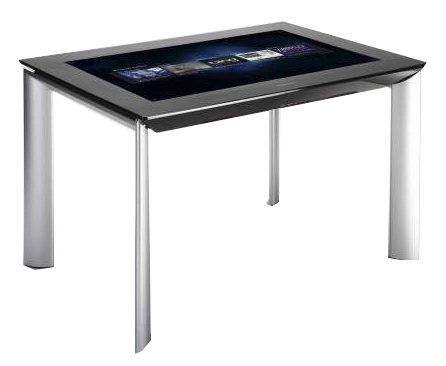
\includegraphics{SUR40.jpg}}
\caption{SUR40 Touchscreen Table}
\label{Fig:table}
\end{figure}

The Pixelsense 2.0 developer packages for the SUR40 had a lot of positives that made it attractive for this project.    The developer tools had a parent classes (ScatterView) and (ScatterViewItem) that gave objects physical properties.  When touched, a shadow was activated to give the illusion of the item being picked up.  ScatterViewItems have built in multi-touch gestures, such as pinch to scale, dragging, and rotations. Additionally, they had inertia, momentum, and a center of mass that allows users to do a one finger rotation as well.  The ScatterView is optimized for ScatterViewItems creating an environment in which they can exist.  ScatterViews have well defined edges that ScatterViewItems cannot cross, instead bouncing off the edge when thrown.  When a ScatterViewItem is places on it, it's rotation and placement is random as to encourage users to stand on any side of the table.  These objects, combined with the C\# wpf framework, minimized the amount of physics that we had to program by hand.

As a stand alone touch screen table, it was designed in such a way as to allow a single user could reach any part of the screen without moving, while still allowing for multiple users simultaneously.  The touchscreen is not capacitive.  Each pixel has an IR Sensor, an RGB Sensor, as well as the pixel.  The table relies on the distance of your hand from the screen as read by the IR sensor to determine whether or not you are touching it.  Additionally, the RGB sensor allows the table can recognize "Microsoft Tags" which are simpler QR codes that can be used for object recognition.  

The fact that the table uses IR sensors expands the realm of interactions.  For example, digital art could be painted with an actual paint brush.  For traditional computing, it gives the user the "hover" state, where the user targets a UI element without activating it, for a 3rd interaction state.  

\section{User Study}
\subsection{Methods}
\subsection*{Subjects}
	Eight Computer Science graduate students between the ages of 22 to 26 from various research specialties participated in this study.  No one had previous experience using Habilis or the SUR40, while six out of eight had no previous experience with Mendeley. All subjects were male with  normal or corrected-to-normal vision with no other known disabilities. 
\subsection*{Equipment}
	Habilis was run on the Samsung SUR40 40-inch touch screen table with no external hardware.  Users were forced to use only touch interactions with a virtual onscreen keyboard. Mendeley was run on a Sony Flip-PC touch screen convertible laptop.  However, no user chose to utilize the touch interactions of the laptop, and instead used a wireless mouse and build in keyboard.  
	
\subsection*{Procedure}

	This experiment was a comparative study between Habilis and Mendeley.  To test which system was better for organizing documents into categories, users were asked to identify citations of a source paper.  We chose to use Bumptop \cite{Agarawala2006}
	as our source paper because it has many sources that neatly divide into several subjects.  The authors also released a seven minute video that gives a detailed overview of all of the features and novel designs without mentioning their sources.   
	
	Bumptop had forty-one sources that encompassed six subjects: advantages of a pile metaphor, stylus interactions, spacial organization, realism, browsing techniques, naive physics, and animation.  Dataset 1 encompassed twenty-one papers covering pile metaphors, stylus interactions, and spacial organization.  The remaining twenty papers went into dataset 2.  Distractor papers were added from mobile and touchscreen research until each dataset had a total of thirty-seven papers.  The subjects were then asked to identify which papers were related to bumptop.  The datasets were alternated between Habilis and Mendeley to overcome any performance bias of the data.  The trials were timed, and at the end they were asked 3 questions:
	\begin{enumerate}
	\item Which system did you prefer? why?
	\item Did you see any topic clusters?  If so, what topics?
	\item What features were you looking for but didn't see in Habilis?
	\end{enumerate}
\section{Results}
\subsection*{Hardware Problems}
Unfortunately, the novel IR technology that this table did not work as well as we had hoped.  In fact, this model was discontinued within a year and a half of it being released because of significant hardware problems.  When sitting in front of the table, it was as likely to read the users wrist as a touch as his or her finger.  When it recognized a "blob" where your palm could be seen, it would register circa 50 events in and around that area.  If there were significant smudges on the table, that could throw off what was happening where your had was.  The most significant problem however, was that the calibration was so sensitive that if the lighting changed at all from when you calibrated it, the table would not function correctly.  This meant that it could not be placed in any room with natural light.  It took us several months to figure out this problem, not realizing that the time of day or the weather could have such a significant impact on the table's usability.  

Once we got the table into a windowless room, we were able to improve many of the problems programmatically within Habilis, but the on screen keyboard continued to be a major problem.  5 of the 8 participants mentioned that they had shied away from using the tools because the keyboard was so hard to use.  Occasionally, a ghost event would make something fly across the screen which would break the user's concentration.  There is no question that the hardware failures contributed to the results of the user study.      
\subsection*{Performance Time}
\subsection*{Number of Incorrect Categorizations}
\subsection*{Questionnaire}
%%RESULTS
%Reaction Time. The main finding in the reaction time data was that the Data Mountain reliably facilitated speedy retrieval of web pages when compared to IE4, allowing users to leverage visual as well as textual cues in finding document locations in 3D space.  Also, the two applications supported different retrieval behaviors.  IE4 leveraged the available textual, title information—any other or additional kind of information that was presented as a retrieval cue had a deleterious effect on performance. For both groups of Data Mountain users, the All cue enabled users to retrieve pages faster than using just a title, indicating that the Data Mountain prototype lets users utilize additional information modalities for improved spatial location memory. Figure 6 shows the results.  Figures 6-8 include error bars showing plus or minus one standard error from the mean. Statistical tests that support these findings are presented next.
%A 3x4 (Application x Cue Condition) analysis of variance (ANOVA) with repeated measures was performed on the reaction time data.  The analysis revealed a statistically reliable main effect of application, F(2,18) =  4.84, p < .02, a statistically reliable effect of cueing condition, F(3,27) = 5.7, p < .01 and a statistically reliable interaction between application and cueing condition, F(6,54) = 3.32, p < .01.  Post hoc analyses (Scheffe tests) revealed that in IE4 the title was the retrieval cue that resulted in the fastest reaction times, reliably faster than either the thumbnail or summary cues (but not reliably faster than the All cue, though this was close to being reliably different).  In the two Data Mountain groups the pattern of results were very different.  Participants were reliably faster, on average, using the Data Mountain, especially in the thumbnail and All cueing conditions.  The only condition in which the first Data Mountain group was slower than the IE4 group was the title cueing condition.  The second Data Mountain group was as fast or faster than the first Data Mountain group and IE4 group in all cueing conditions.
%Number of Incorrect Retrievals. In essence, users performed more accurately with the second Data Mountain. These results are shown in Figure 7.  Statistical analyses supporting these findings are presented next.
%A 3x4 (Application x Cue Condition) ANOVA with repeated measures revealed a statistically reliable main effect of application for number of incorrect pages retrieved, F(2,18) = 4.48, p < .03, as well as a reliable effect of cue, F(3,27) = 7.62, p < .001.  There was also a reliable interaction between application and cueing condition, F(6,54) = 2.4, p < .04.  For the IE4 group incorrect pages were most often visited when the cue was a thumbnail or a summary, while the two Data Mountain groups were only reliably more likely to visit an incorrect page when a summary cue was provided.  Reliably fewer incorrect pages were retrieved in the second Data Mountain group than the other two groups.
%Failed Trials. The two Data Mountain groups were reliably more likely to retrieve a web page within the time limit than the IE4 group.  The IE4 group was more likely to fail trials in either the summary or thumbnail condition, while the Data Mountain groups were more likely to fail trials in the summary condition. This data is shown in Figure 8, with statistical support presented below.
%A 3x4 (Application x Cue Condition) ANOVA with repeated measures revealed reliable main effects of application for the number of trials where the user could not retrieve the page before the two minute deadline, F(2,18) = 8.3, p < .01, as well as a reliable effect of cueing condition, F(3,27) = 46.9, p < .001, and the interaction between application and cue condition, F(6,53) = 19.51, p < .001.
%Subjective Ratings. After completing the retrieval tasks, the participants answered questions about their satisfaction with the application they used in the study.  Table 2 shows the average and standard deviation scores on a five-point scale (1=disagree, 5=agree) for participants’ responses to a number of ease of use and likability ratings.  A one-way analysis of variance was run on each measure to test for differences between the groups.  No reliable main effect was found for any of the ratings.
%One final question was presented for both Data Mountain groups, inquiring whether they would prefer to use IE4 or the Data Mountain software. There was a reliable preference for IE4 in the first Data Mountain group, and eight out of eleven of the second Data Mountain group said they would prefer to use the Data Mountain over IE4 (one participant in the second Data Mountain group failed to answer this question).  This is a statistically reliable preference for the second Data Mountain using a binomial test, and clearly provides converging evidence, beyond the performance data, that iterative testing with end users has improved the user interface of the Data Mountain.


%\subsection*{Failed Trials}
%Table of Questionaire
\section{Discussion \& Future Work}

%\subsection{''subsection''}	2	not in letters
%\subsubsection{''subsubsection''}	3	not in letters

\bibliographystyle{plain}
%\bibliographystyle{acm-sigchi}
\bibliography{890}{}
\end{document}
